% Skeleton for the NeurIPS 2026 main-track paper (venue-repo). Copy next to
% neurips_2026.sty and checklist.tex; do not edit the style file.
% Submission mode: no [final]/[preprint] option -> anonymous, line-numbered.
\documentclass{article}
\usepackage{neurips_2026}

\usepackage[utf8]{inputenc}
\usepackage[T1]{fontenc}
\usepackage{hyperref}
\usepackage{url}
\usepackage{booktabs}
\usepackage{amsfonts,amsmath,amssymb,amsthm}
\usepackage{nicefrac}
\usepackage{microtype}
\usepackage{xcolor}
\usepackage{graphicx}

\newtheorem{proposition}{Proposition}

\title{Can fixed-input prediction-powered intervals be shortened? Headroom, finite-sample cost and validity}

\author{Anonymous Author(s)}

\begin{document}
\maketitle

\begin{abstract}
Prediction-powered inference (PPI, PPI++) gives valid confidence intervals from a small labelled set, a large unlabelled set and a fixed predictor. We ask whether, with all three held fixed and nominal coverage required, these intervals can be shortened, by how much and under what conditions.
Viewing PPI++ as the best control variate that is affine in the predictor, we measure the headroom to the efficiency bound and the finite-sample price of learning a better control variate from the labels, with every width read as a paired ratio against PPI++ calibrated the same way and next to its coverage.
For the mean on seven real pools the headroom, for the adjuster classes we tried, is at most about 1.2\%, and on the four main pools cross-fitted adjusters are significantly wider than PPI++ in 252 of 270 cells for $n\le1000$ (never more than 0.55\% narrower): there, no usable shortening exists.
Where headroom exists, in populations with known truth, it is realised only above a threshold labelled size and by an adjuster matched to it: up to 26\% narrower when the outcome is far from affine in the predictor, and 22\% to 29\% when features carry signal the predictor misses (from $n=50$ with a linear adjuster), at coverage within 1.5 points of PPI++.
For OLS coefficients on census data the gain is 2.8\% at $n=1000$. Under label shift PPI++ and the adjusters lose coverage.
All results come from the released code.
\end{abstract}

\section{Introduction}
\label{sec:intro}
Prediction-powered inference (PPI) turns a small labelled sample and a large unlabelled one, scored by a fixed machine-learning predictor $f$, into a valid confidence interval that is shorter than the labelled-only interval
\citep{angelopoulos2023ppi}; PPI++ tunes the weight of the predictor and is, among corrections that are affine in $f$, the shortest of them \citep{angelopoulos2023ppiplus}.
We ask a question that sits after that: \emph{with the labelled set, the unlabelled set and the predictor all held fixed, and nominal coverage required, can the PPI/PPI++ interval be made shorter, by how much, and under what conditions?}
Nothing is bought here with more labels, a better $f$ or a different labelling design; the only freedom is what the analyst does with the same records.

The answer we find is conditional, and for the most common use it is negative. Writing the estimator as a control variate (Sec.~\ref{sec:theory}), PPI++ is the best affine function of $f$, and a known efficiency bound limits any control variate built from $(f,X)$; the headroom is the gap between the two.
On the seven real pools of the \texttt{ppi-python} package that gap, measured for the adjuster classes we tried (fitted on half-pools, so a lower bound on the true gap), is at most about 1.2\% of the interval width for the mean (Sec.~\ref{sec:headroom}), and learning a better control variate from the $n$ labels costs more than it returns:
of 270 (pool, $n$, adjuster, calibration) cells on the four main pools at $n\le1000$, 252 are significantly \emph{wider} than PPI++ calibrated the same way and none is more than 0.55\% narrower (Sec.~\ref{sec:real}).
Where the headroom is large, which we can only establish in populations with known truth, it is realised, but only above a threshold $n$ and only by an adjuster that matches its shape: up to 26\% narrower when $E[Y|f]$ is far from affine, and
22\% to 29\% when features $X$ carry signal that $f$ misses, for $n$ from 50 (a linear adjuster on $(f,X)$) to several hundred (flexible adjusters), at coverage within 1.5 points of PPI++'s (Sec.~\ref{sec:synth}). On a regression problem with real data (OLS of income on covariates) the saving is 2.8\% at $n=1000$ (Sec.~\ref{sec:ols}).

\paragraph{Contributions.}
(i) A variance calculus that places PPI++ inside a family of cross-fitted control variates, states the efficiency floor for the mean (a known bound, restated) and a first-order account of the estimation cost (Sec.~\ref{sec:theory}).
(ii) A like-for-like protocol: every width is a paired ratio against PPI++ with the same interval calibration (Wald, $t$ or studentised bootstrap) and is read together with coverage and its Wilson interval, because a narrower interval that undercovers is not a saving (Secs.~\ref{sec:method}, \ref{sec:validity}).
(iii) The measured headroom, finite-sample cost and break-even $n$ on the real pools, in synthetic populations whose theory is known, and for OLS coefficients (Secs.~\ref{sec:headroom}--\ref{sec:ols}).
(iv) A statement of when the answer is ``no'' (calibrated or near-affine $f$, no informative $X$, small $n$, label shift) and every cell behind it, with the code that reproduces them.
Positive and negative results are reported with equal weight; the claims are limited to the estimands, adjuster classes and sampling protocol described in Secs.~\ref{sec:method}--\ref{sec:exp} and in the discussion.

\section{Related work}
\label{sec:related}

\paragraph{Prediction-powered inference.}
PPI \citep{angelopoulos2023ppi} combines a small labelled sample with predictions on a large unlabelled one to
obtain valid intervals for means, quantiles and regression coefficients, whatever the predictor. PPI++
\citep{angelopoulos2023ppiplus} tunes the weight placed on the predictions so that the interval is never wider
(asymptotically) than the labelled-only interval, and gives the efficiency bound and equality condition that
frame our question. Variants change what is fixed: cross-prediction-powered inference
\citep{zrnic2023cross} handles predictors trained on the same labelled data by cross-fitting; active statistical
inference \citep{zrnic2024active} chooses which records to label, and stratified PPI \citep{fisch2024stratified}
reweights strata. All of these either add information (a better predictor, a choice of labels) or change the
sampling design. We keep the labelled set, the unlabelled set and the predictor fixed and ask only how
the available information is \emph{used}.

\paragraph{Semi-supervised and doubly-robust inference.}
Semi-supervised estimation of a mean from labelled and unlabelled covariates, with an efficiency bound,
is studied by \citet{zhang2019semisup}, and for linear regression by \citet{chakrabortty2018efficient}.
The cross-fitted, orthogonal-score construction behind our adjusters is that of double/debiased machine learning
\citep{chernozhukov2018dml}. From this view PPI++ is the special case in which the nuisance function is restricted
to be affine in $f$; the question is how much of the remaining distance to the bound can be recovered from the same labelled data,
and at what finite-sample cost. We read the abstracts of the semi-supervised papers and use them for positioning only.

% DRAFT (template-independent body). Numbers are intentionally absent until results/ is final.
\section{Setting and a variance calculus for fixed-input intervals}
\label{sec:theory}

\paragraph{Setting.}
We observe $n$ labelled pairs $(X_i,Y_i)$ and $N$ unlabelled covariates $\tilde X_j$, both i.i.d.\ from the
same population (labels missing completely at random), and a fixed predictor $f$ evaluated on every record, so
every record carries $W=(f(X),X)$. The target is $\theta=\mathbb E[Y]$.
Nothing is added: no labels, no unlabelled records, no change to $f$. Write $\rho=n/N$.

\paragraph{Control-variate form.}
For any fixed $g(W)$ and $\lambda\in\mathbb R$,
\begin{equation}
\hat\theta_{g,\lambda}=\bar Y_n-\lambda\big(\bar g_n-\tilde g_N\big),
\end{equation}
where $\bar g_n$ and $\tilde g_N$ are the means of $g$ on the labelled and unlabelled sets. It is unbiased for
every $\lambda$. Classical inference is $\lambda=0$; PPI \citep{angelopoulos2023ppi} is $g=f,\ \lambda=1$; PPI++
\citep{angelopoulos2023ppiplus} is $g=f$ with $\lambda$ tuned. Hence \emph{PPI++ is the best control variate
affine in $f$}.
Its variance is
\begin{equation}
\mathrm{Var}(\hat\theta_{g,\lambda})=\frac1n\Big[\mathrm{Var}(Y)-2\lambda\,\mathrm{Cov}(Y,g)+\lambda^2(1+\rho)\,\mathrm{Var}(g)\Big],
\end{equation}
minimised at $\lambda^\star=\mathrm{Cov}(Y,g)/\{(1+\rho)\mathrm{Var}(g)\}$, giving
\begin{equation}
\mathrm{Var}^\star(g)=\frac{\mathrm{Var}(Y)}{n}\Big(1-\frac{R_g^2}{1+\rho}\Big),\qquad R_g^2=\mathrm{corr}^2(Y,g(W)).
\label{eq:var}
\end{equation}
\begin{proposition}[Asymptotic width ratio]
For two control variates $g_1,g_2$ the ratio of asymptotic interval widths (same $n$, $N$, level) is
$\sqrt{(1-R_{g_1}^2/(1+\rho))/(1-R_{g_2}^2/(1+\rho))}$.
\end{proposition}
\begin{proposition}[Floor]
For every $g$, $R_g^2\le\eta^2:=\mathrm{Var}(\mathbb E[Y\mid W])/\mathrm{Var}(Y)$, with equality iff $g$ is an
affine function of $\mathbb E[Y\mid W]$. Therefore
$\mathrm{Var}^\star(g)\ge \frac1n\{\mathrm{Var}(Y\mid W)+\tfrac{\rho}{1+\rho}\mathrm{Var}(\mathbb E[Y\mid W])\}
=\mathrm{Var}(Y\mid W)/n+\mathrm{Var}(\mathbb E[Y\mid W])/(n+N)$.
\end{proposition}
The bound is the semiparametric efficiency bound for $\theta$ when labels are missing completely at random and
the unlabelled records reveal only $W$ (nonparametric model for $(W,Y)$). A bound of this form, with the equality
condition that the control variate be proportional to $\mathbb E[Y\mid W]$, is given for general M-estimation
targets by \citet{angelopoulos2023ppiplus}; we restate it for the mean, as a standard result and not as a contribution,
prove the control-variate form of the floor in Appendix~\ref{app:diag} and verify it numerically in Sec.~\ref{sec:exp}. What is new here is the \emph{attainable} part: how close an adjuster
learned from the fixed labelled set gets to the bound, at which $n$, and at what coverage.
\emph{Consequence.} The headroom over PPI++ is exactly $R^2_{\rm aff}\to\eta^2$, where
$R^2_{\rm aff}=\mathrm{corr}^2(Y,f)$ if only $f$ is used. It is zero if $\mathbb E[Y\mid W]$ is affine in $f$ (e.g.\ a
calibrated binary $f$ with no informative $X$). Since $R^2/(1+\rho)$ is what enters~\eqref{eq:var}, the
attainable relative narrowing is largest for small $\rho$ (few labels per unlabelled record) and fades as
$\rho\to\infty$.

\paragraph{Estimating $g$ costs width.}
A richer $g$ must be learned from the same $n$ labels. With $K$-fold cross-fitting, $\hat g^{(-k)}$ is fitted off fold $k$,
so $\hat\theta$ stays unbiased. To first order the variance inflates by the excess risk of $\hat g$:
$\mathrm{Var}(Y-\hat g)\approx\mathrm{Var}(Y-g^\star)+\mathbb E\|\hat g-g^\star\|^2$, so a gain over the affine
tuning needs $(\eta^2-R^2_{\rm aff})\mathrm{Var}(Y)$ to exceed an estimation term that grows with the
adjuster's complexity and shrinks with $n$. This is a heuristic first-order argument, not a theorem: we
use it only to interpret the measured break-even $n$ (Sec.~\ref{sec:exp}) and do not test it as a quantitative prediction.

\paragraph{Intervals.} Wald intervals use the plug-in variance of~\eqref{eq:var}; their coverage is
asymptotic and degrades for skewed or rare-event $Y$ and small $n$. We therefore also use a studentised
bootstrap and always report width next to coverage: a shorter interval that undercovers is not a saving.

\section{Method: cross-fitted control variates and calibrated intervals}
\label{sec:method}

The route we test uses nothing beyond the fixed inputs. It interprets ``predictor fixed'' as: $f$ is not retrained and
no label or unlabelled record is added, but a post-hoc map of $W=(f(X),X)$ fitted on the labelled set is allowed.
Under the control-variate form of Sec.~\ref{sec:theory} this is a choice of $g$. If one insists on $g$ affine in $f$,
the result is PPI++ itself, which is therefore our baseline and the $K\!=\!5$ affine adjuster below is its ablation.

\paragraph{Cross-fitted adjusters.}
Split the labelled set into $K=5$ folds. For each fold $k$ fit an adjuster $\hat g^{(-k)}$ on the other folds, score the held-out
labelled points with it, and score every unlabelled point with the fold average $\bar g_u=K^{-1}\sum_k\hat g^{(-k)}$.
Writing $m_i$ for the out-of-fold score of labelled point $i$,
$\hat\theta=\bar Y_n-\hat\lambda(\bar m_n-\bar g_{u,N})$, with $\hat\lambda$ the plug-in version of $\lambda^\star$
in Sec.~\ref{sec:theory} and variance estimate $\widehat{\mathrm{Var}}(Y-\hat\lambda m)/n+\hat\lambda^2\widehat{\mathrm{Var}}(\bar g_u)/N$.
Because $\hat g^{(-k)}$ never sees the points it scores on the labelled side, the estimator stays centred and the
unlabelled mean is free.
The adjuster classes (all fitted on the labelled set only) are: affine in $f$ (\texttt{lin\_f}); monotone, isotonic in $f$
(\texttt{iso\_f}); cubic polynomial in $f$ (\texttt{poly\_f}); gradient boosting on $f$ (\texttt{gbm\_f}); linear in $(f,X)$
(\texttt{lin\_fX}); gradient boosting on $(f,X)$ (\texttt{gbm\_fX}). Features $X$ exist only for the census pools.

\paragraph{Interval calibration.}
Each estimator has three intervals: Wald ($z_{0.975}$), $t$ with $n-1$ degrees of freedom, and a studentised bootstrap
that resamples labelled pairs $(Y_i,m_i)$, perturbs the unlabelled mean by its normal approximation and re-tunes $\lambda$
in every resample. The same three calibrations are applied to PPI++ ($g=f$). Headline narrowing statements compare an
adjuster with \emph{PPI++ calibrated the same way}, so that a gain from calibrating the interval is not credited to the control variate;
the published practitioner baseline (PPI++, Wald) is reported alongside and flagged wherever it undercovers.

\paragraph{OLS coefficients.}
For the secondary estimand the labelled OLS estimator is corrected by a vector of control variates
$G_i=H^{-1}x_i(m_i-x_i^\top\hat\beta)$, where $H$ is the Gram matrix of all covariates (observed for unlabelled records too)
and $m_i$ imputes $Y_i$ (by $f_i$, or by a cross-fitted adjuster). Each coordinate uses a variance-minimising combination of
either its own control variate (the coordinate-wise PPI++ form) or all $d$ of them. The implementation is checked against
\texttt{ppi\_py} 0.2.3 PPI++.

\section{Experiments}
\label{sec:exp}

\paragraph{Protocol.}
Each repetition draws $n$ labelled and $N$ unlabelled records i.i.d.\ \emph{with replacement} from a pool of
the \texttt{ppi-python} 0.2.3 data (Table~\ref{tab:datasets}); the pool's empirical distribution is the population, so the truth is the pool
mean (for OLS, the pool fit), $Y$ is hidden on the unlabelled draw, and every method sees the same draw (paired comparisons).
Unless stated, $N=\min(\text{pool size},10^4)$ (the validity grid uses $2\times10^4$). Coverage is reported with Wilson 95\% intervals and widths as paired
ratios with confidence intervals; seeds, versions, commands and expected runtimes are in the reproduction notes.
Pools without a population truth or with a shift are used only as stated in the text where they appear.

\begin{table}[t]
\caption{Pools used for the mean. Skewness and $\mathrm{corr}(Y,\hat Y)$ are computed on the full pool; $\dim X$ is the number of
features available to the adjusters.}
\label{tab:datasets}
\centering
\small\begin{tabular}{lrlrrrr}
\toprule
pool & $N_{\mathrm{pool}}$ & outcome & mean $Y$ & skew $Y$ & corr$(Y,\hat Y)$ & $\dim X$ \\
\midrule
galaxies & 16{,}743 & binary & 0.259 & 1.1 & 0.74 & 0 \\
forest & 1{,}596 & binary & 0.152 & 1.9 & 0.54 & 0 \\
alphafold & 10{,}802 & binary & 0.177 & 1.7 & 0.82 & 0 \\
gene\_expression & 61{,}150 & continuous & 6.77 & 0.56 & 0.96 & 0 \\
census\_income & 380{,}091 & continuous & $4.31{\times}10^{4}$ & 4.7 & 0.61 & 2 \\
census\_healthcare & 318{,}215 & binary & 0.671 & $-$0.73 & 0.71 & 2 \\
census\_education & 318{,}215 & continuous & 17.8 & $-$1.8 & 0.63 & 4 \\
\bottomrule
\end{tabular}

\end{table}

\subsection{Validity of the baselines (C0)}
\label{sec:validity}
Width is only meaningful at valid coverage, so we first measure it. Figure~\ref{fig:validity} gives the coverage of nominal 95\%
intervals for classical, PPI and PPI++ (Wald, $t$, studentised bootstrap) on seven pools, 2000 repetitions per cell,
$n\in\{15,25,50,100,200,500\}$.
Wald PPI++ undercovers at small $n$ on skewed or rare-outcome pools: on \texttt{census\_income} its coverage is 0.755 at $n=15$,
0.907 at $n=200$ and 0.926 at $n=500$, and the Monte-Carlo standard error is about 0.5 percentage points at 2000 repetitions. The $t$ quantile
barely helps (0.787, 0.909, 0.928). The studentised bootstrap repairs most of this on \texttt{census\_income} (0.906, 0.929, 0.951) but
over-corrects at $n=15$ on the small, rare-outcome pools (\texttt{forest} 0.658, \texttt{alphafold} 0.698). On the other six pools the shortfall of PPI++ Wald is 1.1 to 7.9 percentage points at $n=50$ and 0 to 2.2 at $n=200$, and at $n=500$ it is
within 1 percentage point of nominal on all six (0.942 to 0.953); \texttt{gene\_expression} is the closest throughout (0.946 at $n=100$). The consequence for what follows is that the useful comparison of widths is \emph{like for like}: an adjuster
is compared with PPI++ calibrated in the same way, and no comparison against an undercovering interval is read as a saving.

\begin{figure}[t]
\centering
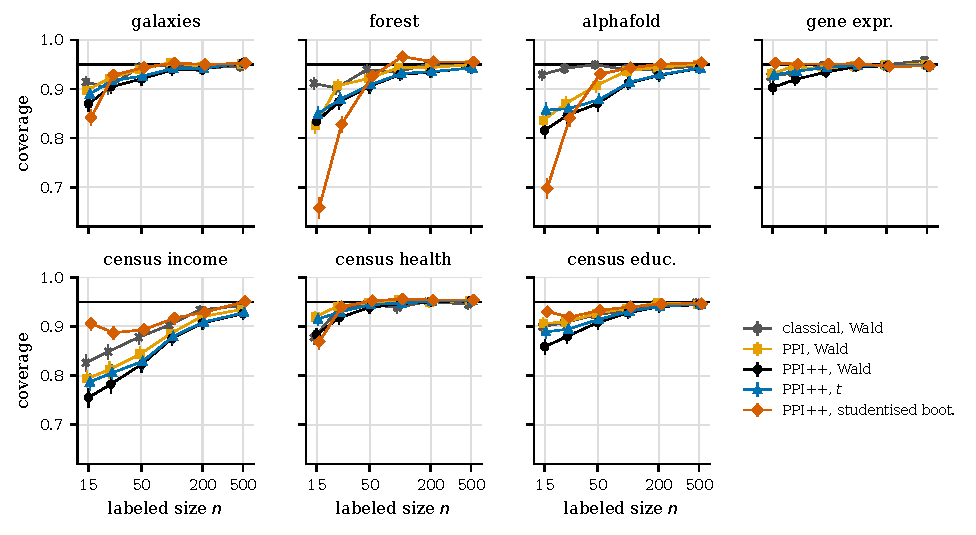
\includegraphics[width=\linewidth]{figures/fig_validity.pdf}
\caption{Coverage of 95\% intervals against labelled size $n$ on seven pools (2000 repetitions per cell; i.i.d.\ with replacement from the pool;
$N=\min(\text{pool},2\times10^4)$; truth = pool mean). Bars: Wilson 95\% intervals; line: nominal level.}
\label{fig:validity}
\end{figure}

\subsection{Population headroom of control variates built from $(f,X)$ (C1)}
\label{sec:headroom}
How much shorter can any adjuster be, if estimated well? Figure~\ref{fig:headroom} shows the asymptotic width ratio
to PPI++ (large $N$) of each adjuster class fitted on the whole pool with 2-fold cross-fitting, with the standard deviation over ten random splits.
On the seven pools the best ratio is 0.988 (\texttt{gene\_expression}, isotonic), 0.995 (\texttt{census\_income}, gradient boosting on $(f,X)$),
0.999 or above elsewhere: at most about 1.2\% in width for the classes tried (a lower bound on the true headroom, since the adjusters are fitted on half-pools), and the best ratio lies inside the grey band of $\pm1\%$ for six of the seven pools. PPI with $\lambda=1$ is
wider than PPI++ on \texttt{gene\_expression} (ratio 1.106) and \texttt{census\_income} (1.022), where $f$ is on a different scale from $Y$; classical
intervals are 1.19 to 3.73 times wider than PPI++. Ratios above one for flexible classes (e.g.\ boosting on \texttt{forest}, 1.021) reflect
the estimation error of an adjuster fitted on half of a 1596-record pool, not a loss of the bound. For the mean on these pools PPI++ is therefore
within about one percent of what any adjuster of the classes tried could reach; whether even that is attainable at the sizes of a labelled set is the
question of the following sections.

\begin{figure}[t]
\centering
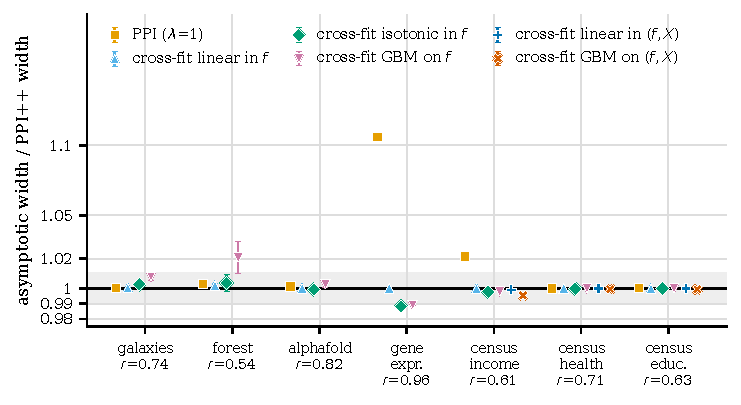
\includegraphics[width=\linewidth]{figures/fig_headroom_population.pdf}
\caption{Population headroom: asymptotic CI-width ratio of the best control variate in each class to power-tuned PPI++ (1 = parity, $<1$ narrower).
Each class is fitted by 2-fold cross-fitting on the full pool; error bars are the standard deviation over ten random splits (split noise only).
Grey band: $\pm1\%$. $r=\mathrm{corr}(Y,f)$.}
\label{fig:headroom}
\end{figure}


\subsection{Finite-sample width and coverage on real pools (C2)}
\label{sec:real}
We now fit the adjusters of Sec.~\ref{sec:method} from the labelled draw only and compare each interval with PPI++ \emph{calibrated the same way} (Wald with Wald, $t$ with $t$, bootstrap with bootstrap), paired
on the same draws. The grid covers the four pools of the main text (\texttt{census\_income}, \texttt{gene\_expression}, \texttt{galaxies}, \texttt{forest}), $n\in\{50,100,200,500,1000\}$ and 2000 repetitions per cell,
with $N=\min(\text{pool},10^4)$; the three further pools are in the appendix. Over all 270 cells (pool, $n$, adjuster, calibration), 252 are significantly
\emph{wider} than the like-for-like PPI++ (the confidence interval of the paired width ratio lies above 1), 9 are indistinguishable from parity and 9 are significantly narrower.
All nine narrower cells are at $n=1000$ on \texttt{forest} (gradient boosting 0.995, isotonic 0.997) and \texttt{gene\_expression} (cubic polynomial 0.998); the largest saving is 0.55\%. The cells are not independent: the three calibrations use the same draws, so the nine are three (pool, adjuster) combinations.
So \emph{on these real pools and for the mean, no adjuster shortens the interval in any practically relevant way}.

\begin{figure}[t]
\centering
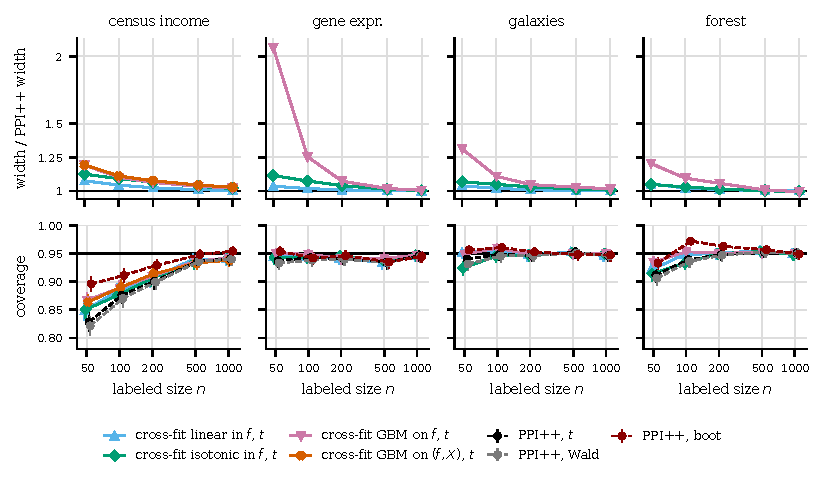
\includegraphics[width=\linewidth]{figures/fig_c2_real.pdf}
\caption{Mean estimation on four real pools. Top: paired width ratio of each cross-fitted adjuster to PPI++ calibrated the same way ($t$ quantile; $<1$ is narrower), geometric mean with 95\% band, log axis; the cubic and the Wald and bootstrap variants are in the delivered summaries. Bottom: coverage of the 95\% interval with Wilson bars; PPI++ (Wald, $t$, bootstrap) dashed.
$n=50$ to $1000$, 2000 repetitions per cell, i.i.d.\ with replacement from the pool, $N=\min(\text{pool},10^4)$, truth the pool mean.}
\label{fig:c2}
\end{figure}

The loss is the estimation cost anticipated in Sec.~\ref{sec:theory} and falls with $n$. At $n=50$ the like-for-like ratios of the affine-in-$f$ adjuster, which is PPI++ up to cross-fitting, are 1.04 to 1.08;
for isotonic recalibration 1.05 to 1.13, for gradient boosting on $f$ 1.20 to 2.06 (\texttt{gene\_expression}). They shrink with $n$ but stay at or above 1.00 for all but the nine cells above (at most 1.03 at $n=1000$).
On \texttt{census\_income}, the pool with features, adjusters that use $X$ do not help: at $n=200$, linear in $(f,X)$ is 1.027 and boosting on $(f,X)$ 1.076, against a population headroom of 0.5\% (Sec.~\ref{sec:headroom}),
which is smaller than the estimation cost, and not recovered within $n\le1000$ (1.005 and 1.027 there). Using studentised bootstrap in place of Wald for both sides gives the same pattern (82 of 90 bootstrap cells significantly wider, 3 narrower).
The same holds as the labelled-to-unlabelled ratio varies: on \texttt{census\_income} at $n=200$ with $N=200$, $2000$ and $20000$, boosting on $(f,X)$ is 1.029, 1.068 and 1.078 times as wide as PPI++, linear in $(f,X)$ 1.010, 1.024 and 1.027;
a larger unlabelled set makes the affine tuning harder to beat, in line with the factor $1/(1+\rho)$ in~\eqref{eq:var}.

\emph{Coverage.} Coverage does not rescue the adjusters: where PPI++ undercovers, the adjusters undercover too, usually slightly less. On \texttt{census\_income} at $n=200$ Wald coverage is 0.899 for PPI++ and 0.902 to 0.912 for the adjusters;
at $n=1000$ 0.940 for PPI++ and 0.938 to 0.943 for the adjusters. Calibrating by the bootstrap lifts PPI++ itself to 0.929 at $n=200$ and 0.954 at $n=1000$, and that calibration is not free: the bootstrap interval for PPI++ is 37\% wider than its Wald interval at $n=50$ and 15\% wider at $n=200$ on \texttt{census\_income}.
The like-for-like comparison is the honest one, since the Wald baseline is narrow partly because it undercovers.
Classical (labelled-only) intervals are 1.1 to 1.5 times wider than PPI++ on \texttt{forest}, \texttt{galaxies} and \texttt{census\_income} at all sizes, and 2.5 to 3.4 times on \texttt{gene\_expression},
so the large gain in this setting is from PPI++'s use of the predictor, not from anything added on top of it.

\subsection{Where headroom exists: synthetic populations with known truth (C3)}
\label{sec:synth}
The real pools leave almost no headroom for the mean, so we ask where shortening is possible at all in populations whose truth and best control variate are known.
$X\sim N(0,I_5)$, $\mu(X)=X_1+\tfrac12X_2$ and $f=\mu(X)$ unless stated. The \emph{knob family} sets $E[Y|f]=\cos\phi\,z+\sin\phi\,(z^2-1)/\sqrt2$ with $z$ the standardised $f$:
$\phi=0^\circ$ is a calibrated predictor (no headroom) and $\phi=90^\circ$ a purely quadratic dependence that no affine map of $f$ can use.
The named scenarios are \texttt{calibrated}; \texttt{heavy\_tail} (calibrated, $t_3$ noise); \texttt{monotone\_miscal} ($E[Y|f]=\mathrm{logit}\,f$ up to scale); \texttt{nonmonotone} ($E[Y|f]=f^2-\mathrm{const}$);
\texttt{X\_informative} ($Y$ depends on a feature $f$ misses); \texttt{subgroup\_bias} ($f$ biased by $+1.5$ on a subgroup);
\texttt{f\_noise\_X\_informative} ($f$ is pure noise, $X$ carries the signal); and \texttt{pure\_noise} (neither carries signal).
We use $n\in\{50,100,200,500,1000\}$ (knobs) or $\{50,200,500\}$ (named), $\rho\in\{1,0.1\}$, and 2000 (knobs) or 1000 (named) repetitions. The \texttt{oracle} control variate uses the true $E[Y|f,X]$; it is not implementable, and is the bound for adjusters of the classes of Sec.~\ref{sec:method}.
Ratios are paired width ratios against Wald PPI++ (Wald against Wald).

\begin{figure}[t]
\centering
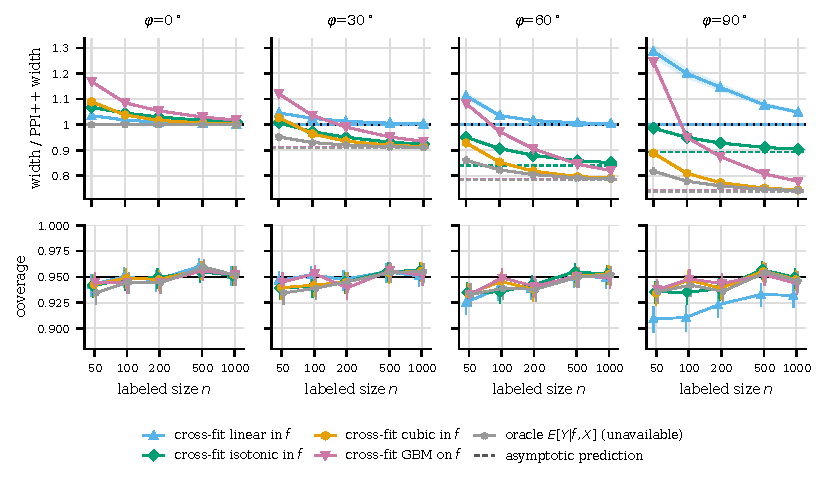
\includegraphics[width=\linewidth]{figures/fig_c3_synth.pdf}
\caption{Knob family at $\rho=0.1$ ($N=10n$), 2000 repetitions per cell, known truth. Top: paired width ratio to Wald PPI++ (solid, 95\% band); dashed horizontal lines: asymptotic prediction for the best adjuster of the class; grey: oracle $E[Y|f,X]$. Bottom: coverage with Wilson bars. The headroom appears only above a threshold $n$ that grows with the flexibility of the adjuster. Other scenarios and $\rho=1$: Appendix~\ref{app:figs}.}
\label{fig:c3}
\end{figure}

\emph{Theory.} The asymptotic ratio of Sec.~\ref{sec:theory} predicts the oracle's measured ratio closely once $n\ge200$: in the 56 cells with $n\ge200$ the measured oracle ratio exceeds the prediction by a median of 0.05\% and at most 6.6\%
(\texttt{nonmonotone}, $\rho=0.1$, $n=200$), and in the 32 cells with $n\le100$ by at most 22.5\% (\texttt{nonmonotone}, $n=50$). For the knobs $\phi=30^\circ,60^\circ,90^\circ$ at $\rho=0.1$, $n=1000$ the oracle is 0.912, 0.788 and 0.743 times as wide as PPI++, against predicted 0.910, 0.784 and 0.738;
at $\rho=1$ it is 0.961, 0.894 and 0.866 against 0.961, 0.894 and 0.866. The attainable saving is thus a property of the population and of $\rho$: up to 26\% at $\rho=0.1$ and 13\% at $\rho=1$ across the knobs.

\emph{What is realised.} The adjuster must match the shape of the headroom and then pay for learning it. In the knob family at $\rho=0.1$ the cubic in $f$ is the first to cross below parity: its ratio at $n=50,100,200,500,1000$ is
$0.929,0.853,0.818,0.797,0.791$ for $\phi=60^\circ$ and $0.888,0.810,0.774,0.752,0.745$ for $\phi=90^\circ$ (oracle 0.788 and 0.743), and 1.027, 0.964, 0.935, 0.919, 0.914 for $\phi=30^\circ$, significantly below 1 from $n=100$.
Gradient boosting on $f$ needs $n\ge100$ to 200 (0.779 at $\phi=90^\circ$, $n=1000$); isotonic regression gains at small $n$ but stalls (0.904 at $\phi=90^\circ$, $n=1000$), since it cannot represent a non-monotone map.
The affine cross-fit, the PPI++ ablation, never gains at $\rho=0.1$ and where the best affine slope is nearly zero it is clearly wider than PPI++ (1.286 at $\phi=90^\circ$, $n=50$, 1.049 at $n=1000$); at $\rho=1$ it stays within 3\% of parity.
At $\phi=0^\circ$ every adjuster is wider than PPI++ at every $n$ (isotonic 1.067, cubic 1.089, boosting 1.168 at $n=50$, $\rho=0.1$; 1.010, 1.003 and 1.018 at $n=1000$).
The named scenarios agree. \texttt{nonmonotone}, $\rho=0.1$, $n=500$: cubic 0.576 (oracle 0.573), boosting on $f$ 0.668, isotonic 0.855, affine 1.092.
\texttt{calibrated} and \texttt{heavy\_tail} have no headroom and no cross-fitted adjuster goes below 1.001 at any $n$, and in \texttt{pure\_noise} the affine cross-fit is 10.5\% and 5.8\% wider than PPI++ at $\rho=0.1$, $n=200$ and $500$ while boosting is at parity (0.999); \texttt{monotone\_miscal} has little (oracle 0.976, 0.963, 0.961 at $n=50,200,500$, $\rho=0.1$), of which the isotonic, cubic and $(f,X)$-linear adjusters reach only a part (0.994, 0.989 and 0.984 at $n=200$).

\emph{Features.} When $X$ carries signal the linear adjuster on $(f,X)$, with $d+2$ parameters, is the practical route. It is significantly narrower than PPI++ already at $n=50$ in \texttt{X\_informative} (0.886 at $\rho=0.1$, 0.947 at $\rho=1$; oracle 0.828, 0.926),
\texttt{subgroup\_bias} (0.950, 0.974; oracle 0.880, 0.946) and \texttt{f\_noise\_X\_informative} (0.777, 0.878; oracle 0.720, 0.853), and at $n=500$, $\rho=0.1$ is within one percentage point of the oracle in all three (0.823, 0.880, 0.711).
Boosting on $(f,X)$ is significantly narrower from $n=200$ in the first two (0.909 at $n=200$ and 0.864 at $n=500$ for \texttt{X\_informative}, $\rho=0.1$) but 2\% to 6\% wider at $n=50$.
In \texttt{f\_noise\_X\_informative} PPI++ is fed a predictor with no information, and looking at $X$ shortens the interval by 22\% to 29\% at $\rho=0.1$ ($n=50$ to $500$): the fixed predictor is what limits PPI++ there, not the estimator.

\emph{Coverage.} For the 36 cells with $n\ge200$ in which \texttt{lin\_fX} or \texttt{poly\_f} is at least 2\% narrower (significantly), Wald coverage is 0.935 to 0.958, between $-1.5$ and $+1.1$ points of PPI++ in the same cell, and only four cells (all $n=200$, cubic) have a Wilson interval that excludes 0.95, all from below (lowest 0.935).
Across all cross-fitted Wald cells coverage is 0.876 to 0.957 at $n=50$ and 0.932 to 0.956 at $n=1000$, against 0.917 to 0.954 and 0.944 to 0.952 for PPI++. The $t$ quantile leaves the ratios unchanged, and the studentised bootstrap moves them by 0.6 points on average (at most 2.9) for the cubic.

\subsection{Regression coefficients on \texttt{census\_income} (C4)}
\label{sec:ols}
The secondary estimand is the OLS coefficient vector of income on the two covariate columns supplied with the pool (no intercept); truth is the pool fit, $N=10^4$, 2000 repetitions per $n\in\{50,100,200,500,1000\}$.
\texttt{cv\_f} is the control variate built from $f$ alone (PPI++ up to cross-fitting); \texttt{cv\_cf\_lin\_fX} and \texttt{cv\_cf\_gbm\_fX} use $(f,X)$; the reference is \texttt{ppi-python}'s \texttt{ppi\_ols\_ci}, which tunes $\lambda$ per coordinate.
Ratios are against that reference (Table~\ref{tab:ols}); where the two coordinates (age, sex) differ, both are given.
\texttt{cv\_f} matches the library within 0.5\% for $n\ge100$ (1.2\% wider at $n=50$). The linear adjuster on $(f,X)$ is 6.2\%, 7.4\% \emph{wider} at $n=50$, 2.1\%, 2.4\% wider at $n=100$, 0.7\%, 0.6\% narrower at $n=200$, and 2.4\% (both coordinates) narrower at $n=500$ and 2.8\% at $n=1000$; the paired CIs exclude 1 at every $n$.
Boosting on $(f,X)$ is wider through $n=500$ (18.3\%, 17.4\% at $n=50$; 8.1\%, 7.5\% at $n=100$; 0.7\%, 0.4\% at $n=500$) and only breaks even at $n=1000$ (0.995, 0.992). The labelled-only interval is 13\% to 27\% wider than PPI++ throughout.
Coverage tracks the library's: at $n=1000$ 0.930 and 0.947 for \texttt{cv\_cf\_lin\_fX} against 0.934 and 0.949 for \texttt{ppi++\_lib}; at $n=50$ and $100$ both undercover the age coefficient (0.818 and 0.851 against 0.797 and 0.844).

\begin{table}[t]
\caption{OLS of income on (age, sex) on \texttt{census\_income}: paired width ratio to \texttt{ppi-python} PPI++ ($<1$ narrower) and coverage of 95\% intervals (Monte-Carlo SE about 0.005); 2000 repetitions, $N=10^4$.}
\label{tab:ols}
\centering
\scriptsize\setlength{\tabcolsep}{3pt}\renewcommand{\arraystretch}{0.84}\begin{tabular}{rlrrrrr|rrrr}
\toprule
 & & \multicolumn{5}{c}{width / PPI++ width} & \multicolumn{4}{|c}{coverage} \\
\cmidrule(lr){3-7}\cmidrule(l){8-11}
$n$ & coef. & classical & PPI & cv.\ $f$ & lin.\ $(f,X)$ & GBM $(f,X)$ & PPI++ & classical & lin.\ $(f,X)$ & GBM $(f,X)$ \\
\midrule
50 & age & 1.268 & 1.002 & 1.007 & 1.062 & 1.183 & 0.797 & 0.840 & 0.819 & 0.849 \\
 & sex & 1.260 & 1.004 & 1.010 & 1.074 & 1.173 & 0.916 & 0.932 & 0.925 & 0.929 \\
100 & age & 1.232 & 1.001 & 1.002 & 1.021 & 1.081 & 0.845 & 0.880 & 0.851 & 0.865 \\
 & sex & 1.220 & 1.002 & 1.002 & 1.024 & 1.075 & 0.929 & 0.938 & 0.934 & 0.930 \\
200 & age & 1.194 & 1.001 & 1.000 & 0.993 & 1.037 & 0.897 & 0.918 & 0.896 & 0.900 \\
 & sex & 1.181 & 1.002 & 1.000 & 0.994 & 1.032 & 0.939 & 0.948 & 0.938 & 0.938 \\
500 & age & 1.163 & 1.001 & 0.999 & 0.976 & 1.007 & 0.913 & 0.918 & 0.918 & 0.917 \\
 & sex & 1.151 & 1.002 & 0.999 & 0.976 & 1.004 & 0.942 & 0.934 & 0.942 & 0.941 \\
1000 & age & 1.145 & 1.001 & 0.999 & 0.972 & 0.995 & 0.934 & 0.938 & 0.930 & 0.931 \\
 & sex & 1.134 & 1.002 & 1.000 & 0.972 & 0.992 & 0.949 & 0.943 & 0.947 & 0.949 \\
\bottomrule
\end{tabular}

\end{table}

On this real regression problem the shortening exists, is below 3\%, and needs $n\ge200$ to $500$ to appear (it is a loss of up to 7\% below that); it is the real-data counterpart of the \texttt{X\_informative} results of the previous subsection, at a much smaller effect.

\section{Discussion and limitations}
\label{sec:discussion}
\paragraph{What the evidence says.}
With inputs fixed, the room to shorten PPI++ is set by how far $E[Y\mid f,X]$ is from affine in $f$, which can be estimated before choosing a method. On the seven real pools it is at most about 1.2\% for the mean for the adjuster classes tried (a lower bound on the true gap), and all but nine of 270 adjuster cells are wider than PPI++ (Sec.~\ref{sec:real}),
so a practitioner with these data should keep PPI++ and, if intervals undercover at small $n$, calibrate them (Sec.~\ref{sec:validity}) rather than add an adjuster. The cases where an adjuster does pay off share two features: a large gap $\eta^2-R^2_{\rm aff}$, and $n$ beyond a threshold set by the adjuster's size ($n=50$ already for a $(d{+}2)$-parameter linear map, a few hundred for boosting).
A cheap diagnostic suggested by the population calculation of Sec.~\ref{sec:headroom}, which we did not evaluate as a decision rule: fit the candidate adjusters by cross-fitting on the labelled set and compare their out-of-fold $R^2$ with that of the affine fit; if the gain in $R^2/(1+\rho)$ is below the estimation cost, expect a loss.
Gains also fade as $\rho$ grows (Sec.~\ref{sec:theory}): a large unlabelled set makes PPI++ harder to beat (Sec.~\ref{sec:real}).

\paragraph{Limitations.}
\emph{Sampling protocol.} Real-pool experiments resample the pool i.i.d.\ with replacement and take the pool mean (or fit) as truth; this is a clean finite population and not a fresh draw from a super-population, and $N\le2\times10^4$ throughout, so small $\rho$ is covered only by the synthetic study and by the sweep at $n=200$ (Sec.~\ref{sec:real}).
\emph{Assumptions.} Labels are missing completely at random, labelled and unlabelled records are exchangeable; under the $2013\to2014$ shift on \texttt{plankton} (Appendix~\ref{app:diag}) PPI++ and the two adjusters tested lose coverage and nothing in this paper repairs it.
\emph{Scope.} Five adjuster classes with default hyper-parameters, $K=5$ folds, mean and OLS only (no quantiles or logistic regression), a binary predictor only in the diagnostics; a better-tuned or richer learner could shift the break-even $n$ but not the floor.
\emph{Theory.} The efficiency floor is a restated, known bound; the estimation-cost argument is first-order and we do not prove a break-even $n$ nor test it quantitatively. \emph{Synthetic scenarios} have headroom by construction and show what is possible, not what is typical.
\emph{Validity.} Wald, $t$ and the bootstrap undercover at small $n$ on skewed or rare-outcome pools (down to 0.755 at $n=15$), and ratios are only read where coverage is comparable; we claim no finite-sample guarantee for any of the intervals.
\emph{Statistical power.} Ratios carry paired confidence intervals; a ratio within 0.5\% of 1 is called parity or a negligible effect, not a finding.
Intervals that are shorter with no loss of coverage are a benefit; we see no harm beyond the stated misuse of narrower-but-undercovering intervals. The census pools are public, anonymised microdata; age and sex enter only as regression covariates, and we infer or release nothing about individuals.


% No acknowledgments / funding text in the anonymous version (use the ack
% environment, which the style file hides when anonymous).

\bibliographystyle{plainnat}
\bibliography{references}   % natbib prints the heading "References"

\appendix
\section{Diagnostics and further results}
\label{app:diag}
\paragraph{Proofs of Propositions 1 and 2.}
Assumptions are those of Sec.~\ref{sec:theory}: i.i.d.\ labelled and unlabelled records, $\mathrm{Var}(Y)<\infty$, $\mathrm{Var}(g(W))\in(0,\infty)$.
\emph{Variance.} The labelled and unlabelled records are independent, so
$\mathrm{Var}(\hat\theta_{g,\lambda})=\mathrm{Var}(Y-\lambda g)/n+\lambda^2\mathrm{Var}(g)/N
=\tfrac1n\{\mathrm{Var}(Y)-2\lambda\mathrm{Cov}(Y,g)+\lambda^2(1+\rho)\mathrm{Var}(g)\}$.
This is a convex quadratic in $\lambda$, minimised at $\lambda^\star=\mathrm{Cov}(Y,g)/\{(1+\rho)\mathrm{Var}(g)\}$, where it equals $\tfrac{\mathrm{Var}(Y)}n\{1-R_g^2/(1+\rho)\}$ (Eq.~\ref{eq:var}).
\emph{Proposition 1.} A Wald interval has half-width proportional to the estimated standard deviation, which is consistent for the square root of the variance above, so by Slutsky's theorem the ratio of two widths converges to the ratio of the square roots of the minimal variances; with Eq.~\eqref{eq:var} for $g_1,g_2$ the common factor $\mathrm{Var}(Y)/n$ and the quantile cancel.
\emph{Proposition 2.} Write $m=\mathbb E[Y\mid W]$ and $V=\mathrm{Var}(m)$, so $\mathrm{Var}(Y)=\mathbb E\,\mathrm{Var}(Y\mid W)+V$ (the term $\mathrm{Var}(Y\mid W)$ in the statement is its expectation). Since $g$ is a function of $W$, $\mathrm{Cov}(Y,g)=\mathrm{Cov}(m,g)$, hence $R_g^2=\mathrm{corr}^2(m,g)\,\eta^2\le\eta^2$ by Cauchy--Schwarz, with equality iff $g$ is almost surely an affine function of $m$.
Substituting $\eta^2$ in Eq.~\eqref{eq:var}: $\mathrm{Var}^\star(g)\ge\tfrac1n\{\mathrm{Var}(Y)-\tfrac{V}{1+\rho}\}=\tfrac1n\{\mathbb E\,\mathrm{Var}(Y\mid W)+\tfrac{\rho}{1+\rho}V\}$, and $\tfrac{\rho}{n(1+\rho)}=\tfrac1{n+N}$ gives the second form. \qed
We do not reprove the statement that the bound is the semiparametric efficiency bound; it is cited as known \citep{angelopoulos2023ppiplus}.

\paragraph{Population headroom per pool and class.}
Table~\ref{tab:headroom} gives the numbers behind Fig.~\ref{fig:headroom} (asymptotic width ratio to PPI++, mean $\pm$ SD over ten 2-fold splits).

\begin{table}[h]
\caption{Asymptotic CI-width ratio to power-tuned PPI++ ($N\to\infty$; 1 = parity, $<1$ narrower) per pool and control-variate class; mean $\pm$ SD over ten random 2-fold cross-fitting splits. ``--'': no features $X$ in the pool.}
\label{tab:headroom}
\centering
\scriptsize\setlength{\tabcolsep}{3pt}\begin{tabular}{lrrrrrr}
\toprule
pool & PPI & lin.\ $f$ & isot.\ $f$ & GBM $f$ & lin.\ $(f,X)$ & GBM $(f,X)$ \\
\midrule
galaxies & $1.000{\pm}.000$ & $1.000{\pm}.000$ & $1.003{\pm}.001$ & $1.008{\pm}.002$ & -- & -- \\
forest & $1.003{\pm}.000$ & $1.002{\pm}.002$ & $1.004{\pm}.005$ & $1.021{\pm}.011$ & -- & -- \\
alphafold & $1.001{\pm}.000$ & $1.000{\pm}.000$ & $0.999{\pm}.001$ & $1.003{\pm}.002$ & -- & -- \\
gene\_expression & $1.106{\pm}.000$ & $1.000{\pm}.000$ & $0.988{\pm}.000$ & $0.989{\pm}.001$ & -- & -- \\
census\_income & $1.022{\pm}.000$ & $1.000{\pm}.000$ & $0.998{\pm}.000$ & $0.998{\pm}.000$ & $0.999{\pm}.000$ & $0.995{\pm}.000$ \\
census\_healthcare & $1.000{\pm}.000$ & $1.000{\pm}.000$ & $1.000{\pm}.000$ & $1.000{\pm}.000$ & $1.000{\pm}.000$ & $1.000{\pm}.000$ \\
census\_education & $1.000{\pm}.000$ & $1.000{\pm}.000$ & $1.000{\pm}.000$ & $1.000{\pm}.000$ & $1.000{\pm}.000$ & $0.999{\pm}.000$ \\
\bottomrule
\end{tabular}

\end{table}

\paragraph{Label shift (\texttt{plankton}).}
The predictor is binary. Without shift (labelled and unlabelled drawn from the 2013 pool, $N=10^4$, 2000 repetitions) the like-for-like ratio of the cross-fitted affine and isotonic adjusters is 1.215 and 1.267 at $n=25$, 1.039 at $n=100$ and 1.003 at $n=1000$, and PPI++ covers 0.856, 0.911 and 0.943 at those sizes: the same picture as Sec.~\ref{sec:real}.
Under the stress test (labelled from 2013, unlabelled from 2014, truth the 2014 mean of $Y$), the exchangeability assumption fails: PPI++ covers 0.741 at $n=100$, 0.607 at $n=200$ and 0.349 at $n=1000$, the two adjusters 0.768/0.768, 0.622/0.624 and 0.352/0.358, and the labelled-only interval 0.000 at $n=1000$.
PPI with $\lambda=1$ covers 0.952, 0.944 and 0.946 at the same sizes; we did not isolate why, but it is consistent with power-tuning shifting weight toward the biased labelled mean. In this regime a shorter interval is not a saving because no interval tested is valid; we have no remedy.

\paragraph{Unlabelled records without outcomes (\texttt{ballots}).}
Only the 1027 labelled ballots have a truth, so two diagnostics are run. \emph{Subsample}: $n$ labelled drawn without replacement from the 1027 and the rest as unlabelled; truth is the 1027-ballot mean. Coverage is 0.98 to 1.00 for PPI++ at $n\ge25$ (the finite population fixes the truth; this is not a validity test of the i.i.d.\ theory) and the adjusters are 0.0\% to 2.2\% wider.
\emph{Width only}: unlabelled are the $78{,}150$ ballots with predictions only. The isotonic adjuster is 2.4\%, 2.1\%, 1.7\%, 1.2\% and 0.6\% wider than PPI++ at $n=25,50,100,200,400$, and the labelled-only interval is 5.0 to 11 times wider. No coverage is claimed.

\paragraph{Further figures.}\label{app:figs}
Figures~\ref{fig:app_c2}--\ref{fig:app_named_b} extend Figs.~\ref{fig:c2} and~\ref{fig:c3} and follow the same layout (paired like-for-like width ratio above, coverage below).
\begin{figure}[h]
\centering
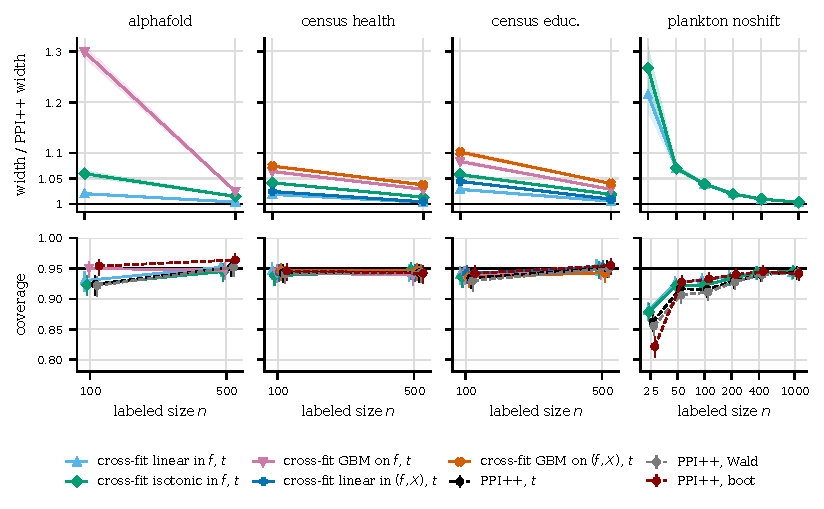
\includegraphics[width=\linewidth]{figures/fig_c2_real_app_a.pdf}
\caption{Mean estimation on \texttt{alphafold}, \texttt{census\_healthcare}, \texttt{census\_education} ($n=100,500$, 1000 repetitions) and on \texttt{plankton} without shift ($n$ from 25 to 1000, 2000 repetitions).}
\label{fig:app_c2}
\end{figure}
\begin{figure}[h]
\centering
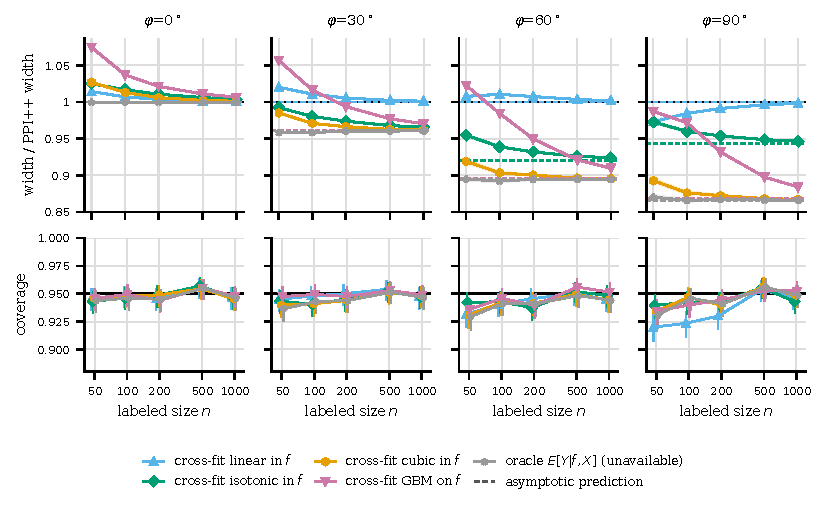
\includegraphics[width=\linewidth]{figures/fig_c3_synth_app_knob_rho1.pdf}
\caption{Knob family at $\rho=1$ ($N=n$), 2000 repetitions per cell.}
\label{fig:app_knob1}
\end{figure}
\begin{figure}[h]
\centering
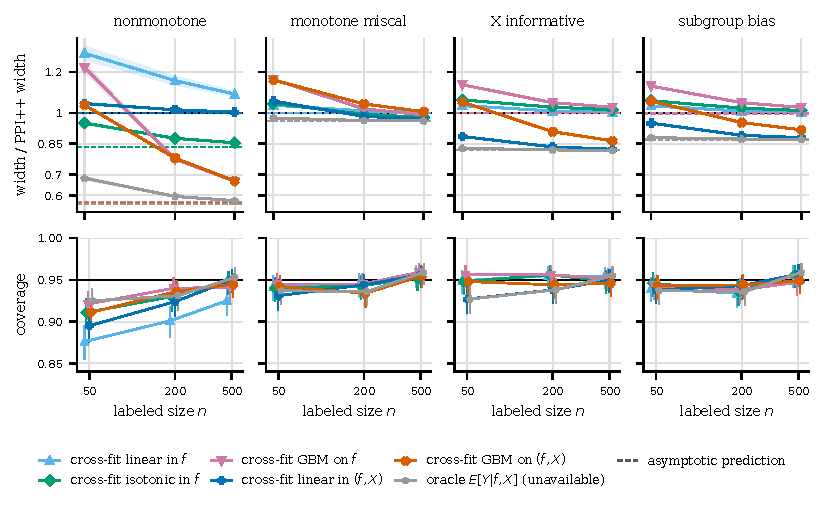
\includegraphics[width=\linewidth]{figures/fig_c3_synth_app_named_a_rho0.1.pdf}
\caption{\texttt{nonmonotone}, \texttt{monotone\_miscal}, \texttt{X\_informative}, \texttt{subgroup\_bias} at $\rho=0.1$, 1000 repetitions per cell, with the $(f,X)$ adjusters.}
\label{fig:app_named_a}
\end{figure}
\begin{figure}[h]
\centering
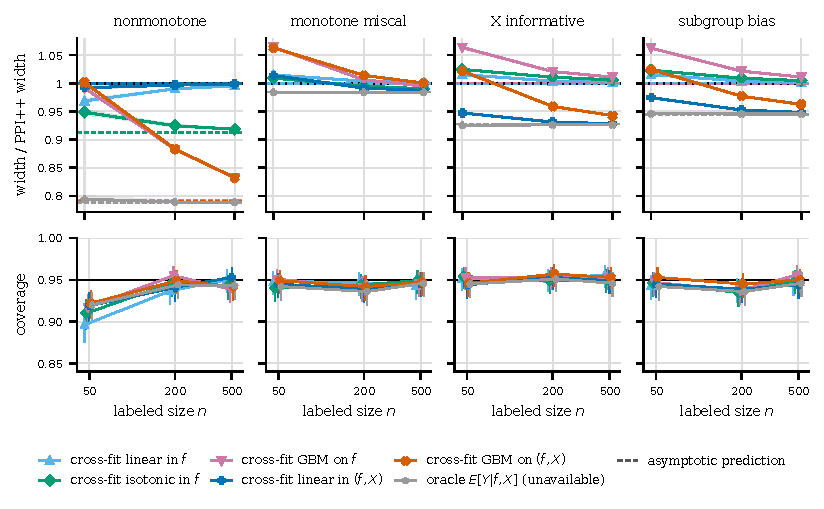
\includegraphics[width=\linewidth]{figures/fig_c3_synth_app_named_a_rho1.pdf}
\caption{As Fig.~\ref{fig:app_named_a} at $\rho=1$.}
\end{figure}
\begin{figure}[h]
\centering
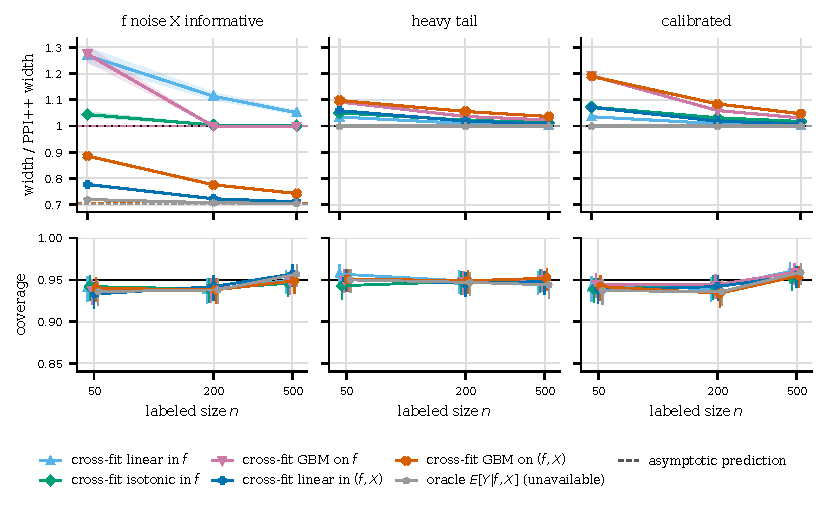
\includegraphics[width=\linewidth]{figures/fig_c3_synth_app_named_b_rho0.1.pdf}
\caption{\texttt{f\_noise\_X\_informative}, \texttt{heavy\_tail}, \texttt{calibrated} at $\rho=0.1$, 1000 repetitions per cell.}
\label{fig:app_named_b}
\end{figure}
\begin{figure}[h]
\centering
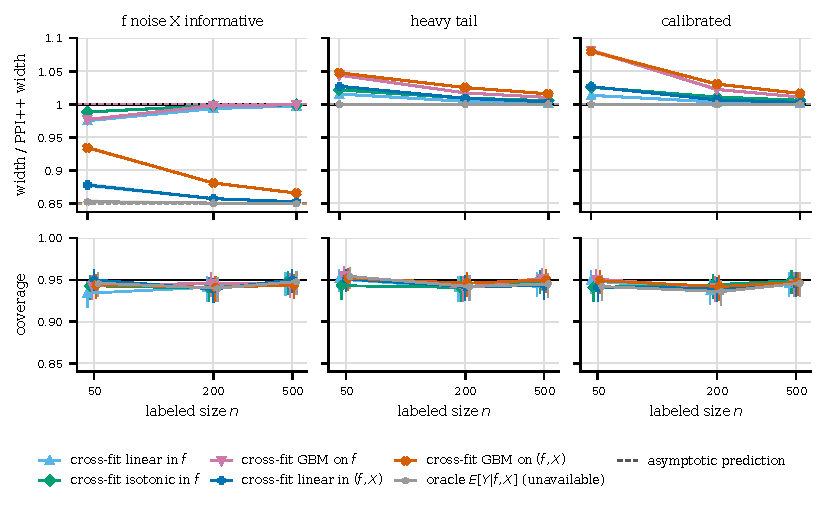
\includegraphics[width=\linewidth]{figures/fig_c3_synth_app_named_b_rho1.pdf}
\caption{As Fig.~\ref{fig:app_named_b} at $\rho=1$.}
\end{figure}


\newpage
\section*{NeurIPS Paper Checklist}



\begin{enumerate}

\item {\bf Claims}
    \item[] Question: Do the main claims made in the abstract and introduction accurately reflect the paper's contributions and scope?
    \item[] Answer: \answerYes{}
    \item[] Justification: Abstract and Sec.~\ref{sec:intro} state the conditional answer: no usable shortening for the mean on the real pools, shortening up to 26\% (29\% with informative features) only where headroom and sufficient $n$ exist, and a 2.8\% gain for OLS; scope and limits are in Sec.~\ref{sec:discussion}.
    \item[] Guidelines:
    \begin{itemize}
        \item The answer \answerNA{} means that the abstract and introduction do not include the claims made in the paper.
        \item The abstract and/or introduction should clearly state the claims made, including the contributions made in the paper and important assumptions and limitations. A \answerNo{} or \answerNA{} answer to this question will not be perceived well by the reviewers. 
        \item The claims made should match theoretical and experimental results, and reflect how much the results can be expected to generalize to other settings. 
        \item It is fine to include aspirational goals as motivation as long as it is clear that these goals are not attained by the paper. 
    \end{itemize}

\item {\bf Limitations}
    \item[] Question: Does the paper discuss the limitations of the work performed by the authors?
    \item[] Answer: \answerYes{}
    \item[] Justification: Sec.~\ref{sec:discussion} (Discussion and limitations) lists the sampling protocol, the i.i.d./MCAR assumptions, the label-shift failure, adjuster classes, estimands, the untested first-order cost argument and the undercoverage of all intervals at small $n$.
    \item[] Guidelines:
    \begin{itemize}
        \item The answer \answerNA{} means that the paper has no limitation while the answer \answerNo{} means that the paper has limitations, but those are not discussed in the paper. 
        \item The authors are encouraged to create a separate ``Limitations'' section in their paper.
        \item The paper should point out any strong assumptions and how robust the results are to violations of these assumptions (e.g., independence assumptions, noiseless settings, model well-specification, asymptotic approximations only holding locally). The authors should reflect on how these assumptions might be violated in practice and what the implications would be.
        \item The authors should reflect on the scope of the claims made, e.g., if the approach was only tested on a few datasets or with a few runs. In general, empirical results often depend on implicit assumptions, which should be articulated.
        \item The authors should reflect on the factors that influence the performance of the approach. For example, a facial recognition algorithm may perform poorly when image resolution is low or images are taken in low lighting. Or a speech-to-text system might not be used reliably to provide closed captions for online lectures because it fails to handle technical jargon.
        \item The authors should discuss the computational efficiency of the proposed algorithms and how they scale with dataset size.
        \item If applicable, the authors should discuss possible limitations of their approach to address problems of privacy and fairness.
        \item While the authors might fear that complete honesty about limitations might be used by reviewers as grounds for rejection, a worse outcome might be that reviewers discover limitations that aren't acknowledged in the paper. The authors should use their best judgment and recognize that individual actions in favor of transparency play an important role in developing norms that preserve the integrity of the community. Reviewers will be specifically instructed to not penalize honesty concerning limitations.
    \end{itemize}

\item {\bf Theory assumptions and proofs}
    \item[] Question: For each theoretical result, does the paper provide the full set of assumptions and a complete (and correct) proof?
    \item[] Answer: \answerYes{}
    \item[] Justification: Sec.~\ref{sec:theory} states the setting (i.i.d., labels missing completely at random) and the two propositions, which are proved in Appendix~\ref{app:diag} from the control-variate variance formula; the efficiency floor is a known bound and is restated as such, and the estimation-cost argument is labelled a heuristic, not a theorem.
    \item[] Guidelines:
    \begin{itemize}
        \item The answer \answerNA{} means that the paper does not include theoretical results. 
        \item All the theorems, formulas, and proofs in the paper should be numbered and cross-referenced.
        \item All assumptions should be clearly stated or referenced in the statement of any theorems.
        \item The proofs can either appear in the main paper or the supplemental material, but if they appear in the supplemental material, the authors are encouraged to provide a short proof sketch to provide intuition. 
        \item Inversely, any informal proof provided in the core of the paper should be complemented by formal proofs provided in appendix or supplemental material.
        \item Theorems and Lemmas that the proof relies upon should be properly referenced. 
    \end{itemize}

    \item {\bf Experimental result reproducibility}
    \item[] Question: Does the paper fully disclose all the information needed to reproduce the main experimental results of the paper to the extent that it affects the main claims and/or conclusions of the paper (regardless of whether the code and data are provided or not)?
    \item[] Answer: \answerYes{}
    \item[] Justification: Secs.~\ref{sec:method} and \ref{sec:exp} give the estimators, adjuster classes, folds, calibrations, sampling protocol, $n$, $N$, repetitions and truths; the reproduction notes (\texttt{README.md}) give versions, data steps, seeds, commands and runtimes.
    \item[] Guidelines:
    \begin{itemize}
        \item The answer \answerNA{} means that the paper does not include experiments.
        \item If the paper includes experiments, a \answerNo{} answer to this question will not be perceived well by the reviewers: Making the paper reproducible is important, regardless of whether the code and data are provided or not.
        \item If the contribution is a dataset and\slash or model, the authors should describe the steps taken to make their results reproducible or verifiable. 
        \item Depending on the contribution, reproducibility can be accomplished in various ways. For example, if the contribution is a novel architecture, describing the architecture fully might suffice, or if the contribution is a specific model and empirical evaluation, it may be necessary to either make it possible for others to replicate the model with the same dataset, or provide access to the model. In general. releasing code and data is often one good way to accomplish this, but reproducibility can also be provided via detailed instructions for how to replicate the results, access to a hosted model (e.g., in the case of a large language model), releasing of a model checkpoint, or other means that are appropriate to the research performed.
        \item While NeurIPS does not require releasing code, the conference does require all submissions to provide some reasonable avenue for reproducibility, which may depend on the nature of the contribution. For example
        \begin{enumerate}
            \item If the contribution is primarily a new algorithm, the paper should make it clear how to reproduce that algorithm.
            \item If the contribution is primarily a new model architecture, the paper should describe the architecture clearly and fully.
            \item If the contribution is a new model (e.g., a large language model), then there should either be a way to access this model for reproducing the results or a way to reproduce the model (e.g., with an open-source dataset or instructions for how to construct the dataset).
            \item We recognize that reproducibility may be tricky in some cases, in which case authors are welcome to describe the particular way they provide for reproducibility. In the case of closed-source models, it may be that access to the model is limited in some way (e.g., to registered users), but it should be possible for other researchers to have some path to reproducing or verifying the results.
        \end{enumerate}
    \end{itemize}


\item {\bf Open access to data and code}
    \item[] Question: Does the paper provide open access to the data and code, with sufficient instructions to faithfully reproduce the main experimental results, as described in supplemental material?
    \item[] Answer: \answerYes{}
    \item[] Justification: Code, summarised results and the reproduction notes are supplied with the submission (\texttt{code/}, \texttt{results/}, \texttt{README.md}); the data are the public \texttt{ppi-python} 0.2.3 files, and the synthetic data are generated by the supplied code.
    \item[] Guidelines:
    \begin{itemize}
        \item The answer \answerNA{} means that paper does not include experiments requiring code.
        \item Please see the NeurIPS code and data submission guidelines (\url{https://neurips.cc/public/guides/CodeSubmissionPolicy}) for more details.
        \item While we encourage the release of code and data, we understand that this might not be possible, so \answerNo{} is an acceptable answer. Papers cannot be rejected simply for not including code, unless this is central to the contribution (e.g., for a new open-source benchmark).
        \item The instructions should contain the exact command and environment needed to run to reproduce the results. See the NeurIPS code and data submission guidelines (\url{https://neurips.cc/public/guides/CodeSubmissionPolicy}) for more details.
        \item The authors should provide instructions on data access and preparation, including how to access the raw data, preprocessed data, intermediate data, and generated data, etc.
        \item The authors should provide scripts to reproduce all experimental results for the new proposed method and baselines. If only a subset of experiments are reproducible, they should state which ones are omitted from the script and why.
        \item At submission time, to preserve anonymity, the authors should release anonymized versions (if applicable).
        \item Providing as much information as possible in supplemental material (appended to the paper) is recommended, but including URLs to data and code is permitted.
    \end{itemize}


\item {\bf Experimental setting/details}
    \item[] Question: Does the paper specify all the training and test details (e.g., data splits, hyperparameters, how they were chosen, type of optimizer) necessary to understand the results?
    \item[] Answer: \answerYes{}
    \item[] Justification: Sec.~\ref{sec:exp}: sampling protocol, $K=5$ folds, adjuster classes and the three calibrations are specified; learners use library defaults and no hyper-parameters were tuned on the evaluation data (see \texttt{code/civ.py}); there is no training/test split because the pool is the population.
    \item[] Guidelines:
    \begin{itemize}
        \item The answer \answerNA{} means that the paper does not include experiments.
        \item The experimental setting should be presented in the core of the paper to a level of detail that is necessary to appreciate the results and make sense of them.
        \item The full details can be provided either with the code, in appendix, or as supplemental material.
    \end{itemize}

\item {\bf Experiment statistical significance}
    \item[] Question: Does the paper report error bars suitably and correctly defined or other appropriate information about the statistical significance of the experiments?
    \item[] Answer: \answerYes{}
    \item[] Justification: Coverage is reported with Wilson 95\% intervals and widths as paired ratios with confidence intervals over 1000--2000 repetitions per cell; Monte-Carlo standard errors are stated in the captions and text (Secs.~\ref{sec:validity}--\ref{sec:ols}).
    \item[] Guidelines:
    \begin{itemize}
        \item The answer \answerNA{} means that the paper does not include experiments.
        \item The authors should answer \answerYes{} if the results are accompanied by error bars, confidence intervals, or statistical significance tests, at least for the experiments that support the main claims of the paper.
        \item The factors of variability that the error bars are capturing should be clearly stated (for example, train/test split, initialization, random drawing of some parameter, or overall run with given experimental conditions).
        \item The method for calculating the error bars should be explained (closed form formula, call to a library function, bootstrap, etc.)
        \item The assumptions made should be given (e.g., Normally distributed errors).
        \item It should be clear whether the error bar is the standard deviation or the standard error of the mean.
        \item It is OK to report 1-sigma error bars, but one should state it. The authors should preferably report a 2-sigma error bar than state that they have a 96\% CI, if the hypothesis of Normality of errors is not verified.
        \item For asymmetric distributions, the authors should be careful not to show in tables or figures symmetric error bars that would yield results that are out of range (e.g., negative error rates).
        \item If error bars are reported in tables or plots, the authors should explain in the text how they were calculated and reference the corresponding figures or tables in the text.
    \end{itemize}

\item {\bf Experiments compute resources}
    \item[] Question: For each experiment, does the paper provide sufficient information on the computer resources (type of compute workers, memory, time of execution) needed to reproduce the experiments?
    \item[] Answer: \answerYes{}
    \item[] Justification: The reproduction notes give the CPU-only environment (2 cores suffice), and indicative wall-clock times per grid; no GPU was used.
    \item[] Guidelines:
    \begin{itemize}
        \item The answer \answerNA{} means that the paper does not include experiments.
        \item The paper should indicate the type of compute workers CPU or GPU, internal cluster, or cloud provider, including relevant memory and storage.
        \item The paper should provide the amount of compute required for each of the individual experimental runs as well as estimate the total compute. 
        \item The paper should disclose whether the full research project required more compute than the experiments reported in the paper (e.g., preliminary or failed experiments that didn't make it into the paper). 
    \end{itemize}
    
\item {\bf Code of ethics}
    \item[] Question: Does the research conducted in the paper conform, in every respect, with the NeurIPS Code of Ethics \url{https://neurips.cc/public/EthicsGuidelines}?
    \item[] Answer: \answerYes{}
    \item[] Justification: Public, anonymised census microdata and simulations only; age and sex are used solely as regression covariates, nothing about individuals is inferred or released, and we do no human-subjects work.
    \item[] Guidelines:
    \begin{itemize}
        \item The answer \answerNA{} means that the authors have not reviewed the NeurIPS Code of Ethics.
        \item If the authors answer \answerNo, they should explain the special circumstances that require a deviation from the Code of Ethics.
        \item The authors should make sure to preserve anonymity (e.g., if there is a special consideration due to laws or regulations in their jurisdiction).
    \end{itemize}


\item {\bf Broader impacts}
    \item[] Question: Does the paper discuss both potential positive societal impacts and negative societal impacts of the work performed?
    \item[] Answer: \answerYes{}
    \item[] Justification: Sec.~\ref{sec:discussion}: shorter intervals at nominal coverage are a benefit; the main risk is reading a narrower interval that undercovers as a saving, which the like-for-like protocol is designed to prevent; we foresee no direct negative societal impact.
    \item[] Guidelines:
    \begin{itemize}
        \item The answer \answerNA{} means that there is no societal impact of the work performed.
        \item If the authors answer \answerNA{} or \answerNo, they should explain why their work has no societal impact or why the paper does not address societal impact.
        \item Examples of negative societal impacts include potential malicious or unintended uses (e.g., disinformation, generating fake profiles, surveillance), fairness considerations (e.g., deployment of technologies that could make decisions that unfairly impact specific groups), privacy considerations, and security considerations.
        \item The conference expects that many papers will be foundational research and not tied to particular applications, let alone deployments. However, if there is a direct path to any negative applications, the authors should point it out. For example, it is legitimate to point out that an improvement in the quality of generative models could be used to generate Deepfakes for disinformation. On the other hand, it is not needed to point out that a generic algorithm for optimizing neural networks could enable people to train models that generate Deepfakes faster.
        \item The authors should consider possible harms that could arise when the technology is being used as intended and functioning correctly, harms that could arise when the technology is being used as intended but gives incorrect results, and harms following from (intentional or unintentional) misuse of the technology.
        \item If there are negative societal impacts, the authors could also discuss possible mitigation strategies (e.g., gated release of models, providing defenses in addition to attacks, mechanisms for monitoring misuse, mechanisms to monitor how a system learns from feedback over time, improving the efficiency and accessibility of ML).
    \end{itemize}
    
\item {\bf Safeguards}
    \item[] Question: Does the paper describe safeguards that have been put in place for responsible release of data or models that have a high risk for misuse (e.g., pre-trained language models, image generators, or scraped datasets)?
    \item[] Answer: \answerNA{}
    \item[] Justification: The paper releases no model or data with a risk of misuse.
    \item[] Guidelines:
    \begin{itemize}
        \item The answer \answerNA{} means that the paper poses no such risks.
        \item Released models that have a high risk for misuse or dual-use should be released with necessary safeguards to allow for controlled use of the model, for example by requiring that users adhere to usage guidelines or restrictions to access the model or implementing safety filters. 
        \item Datasets that have been scraped from the Internet could pose safety risks. The authors should describe how they avoided releasing unsafe images.
        \item We recognize that providing effective safeguards is challenging, and many papers do not require this, but we encourage authors to take this into account and make a best faith effort.
    \end{itemize}

\item {\bf Licenses for existing assets}
    \item[] Question: Are the creators or original owners of assets (e.g., code, data, models), used in the paper, properly credited and are the license and terms of use explicitly mentioned and properly respected?
    \item[] Answer: \answerYes{}
    \item[] Justification: \texttt{ppi-python} 0.2.3 and its data (Angelopoulos et al.) are cited and their version stated; the data files carry no separate licence declaration, which we note in the reproduction notes.
    \item[] Guidelines:
    \begin{itemize}
        \item The answer \answerNA{} means that the paper does not use existing assets.
        \item The authors should cite the original paper that produced the code package or dataset.
        \item The authors should state which version of the asset is used and, if possible, include a URL.
        \item The name of the license (e.g., CC-BY 4.0) should be included for each asset.
        \item For scraped data from a particular source (e.g., website), the copyright and terms of service of that source should be provided.
        \item If assets are released, the license, copyright information, and terms of use in the package should be provided. For popular datasets, \url{paperswithcode.com/datasets} has curated licenses for some datasets. Their licensing guide can help determine the license of a dataset.
        \item For existing datasets that are re-packaged, both the original license and the license of the derived asset (if it has changed) should be provided.
        \item If this information is not available online, the authors are encouraged to reach out to the asset's creators.
    \end{itemize}

\item {\bf New assets}
    \item[] Question: Are new assets introduced in the paper well documented and is the documentation provided alongside the assets?
    \item[] Answer: \answerYes{}
    \item[] Justification: The new assets are the code, the summarised results and the reproduction notes (\texttt{README.md}, \texttt{results/PROVENANCE.md}), which document each file and the command that produced it.
    \item[] Guidelines:
    \begin{itemize}
        \item The answer \answerNA{} means that the paper does not release new assets.
        \item Researchers should communicate the details of the dataset\slash code\slash model as part of their submissions via structured templates. This includes details about training, license, limitations, etc. 
        \item The paper should discuss whether and how consent was obtained from people whose asset is used.
        \item At submission time, remember to anonymize your assets (if applicable). You can either create an anonymized URL or include an anonymized zip file.
    \end{itemize}

\item {\bf Crowdsourcing and research with human subjects}
    \item[] Question: For crowdsourcing experiments and research with human subjects, does the paper include the full text of instructions given to participants and screenshots, if applicable, as well as details about compensation (if any)? 
    \item[] Answer: \answerNA{}
    \item[] Justification: No crowdsourcing or human-subject research.
    \item[] Guidelines:
    \begin{itemize}
        \item The answer \answerNA{} means that the paper does not involve crowdsourcing nor research with human subjects.
        \item Including this information in the supplemental material is fine, but if the main contribution of the paper involves human subjects, then as much detail as possible should be included in the main paper. 
        \item According to the NeurIPS Code of Ethics, workers involved in data collection, curation, or other labor should be paid at least the minimum wage in the country of the data collector. 
    \end{itemize}

\item {\bf Institutional review board (IRB) approvals or equivalent for research with human subjects}
    \item[] Question: Does the paper describe potential risks incurred by study participants, whether such risks were disclosed to the subjects, and whether Institutional Review Board (IRB) approvals (or an equivalent approval/review based on the requirements of your country or institution) were obtained?
    \item[] Answer: \answerNA{}
    \item[] Justification: No human subjects, so no IRB approval is needed.
    \item[] Guidelines:
    \begin{itemize}
        \item The answer \answerNA{} means that the paper does not involve crowdsourcing nor research with human subjects.
        \item Depending on the country in which research is conducted, IRB approval (or equivalent) may be required for any human subjects research. If you obtained IRB approval, you should clearly state this in the paper. 
        \item We recognize that the procedures for this may vary significantly between institutions and locations, and we expect authors to adhere to the NeurIPS Code of Ethics and the guidelines for their institution. 
        \item For initial submissions, do not include any information that would break anonymity (if applicable), such as the institution conducting the review.
    \end{itemize}

\item {\bf Declaration of LLM usage}
    \item[] Question: Does the paper describe the usage of LLMs if it is an important, original, or non-standard component of the core methods in this research? Note that if the LLM is used only for writing, editing, or formatting purposes and does \emph{not} impact the core methodology, scientific rigor, or originality of the research, declaration is not required.
    %this research? 
    \item[] Answer: \answerYes{}
    \item[] Justification: The study design, code and text were produced with LLM-based agents; this is not a component of the proposed method (which is classical statistics), and all numbers come from the supplied code.
    \item[] Guidelines:
    \begin{itemize}
        \item The answer \answerNA{} means that the core method development in this research does not involve LLMs as any important, original, or non-standard components.
        \item Please refer to our LLM policy in the NeurIPS handbook for what should or should not be described.
    \end{itemize}

\end{enumerate}   % completed NeurIPS checklist, after references/appendix
\end{document}
